\let\negmedspace\undefined
\let\negthickspace\undefined
\documentclass[journal]{IEEEtran}
\usepackage[a5paper, margin=10mm, onecolumn]{geometry}
%\usepackage{lmodern} % Ensure lmodern is loaded for pdflatex
\usepackage{tfrupee} % Include tfrupee package

\setlength{\headheight}{1cm} % Set the height of the header box
\setlength{\headsep}{0mm}     % Set the distance between the header box and the top of the text

\usepackage{gvv-book}
\usepackage{gvv}
\usepackage{cite}
\usepackage{amsmath,amssymb,amsfonts,amsthm}
\usepackage{algorithmic}
\usepackage{graphicx}
\usepackage{textcomp}
\usepackage{xcolor}
\usepackage{txfonts}
\usepackage{listings}
\usepackage{enumitem}
\usepackage{mathtools}
\usepackage{gensymb}
\usepackage{comment}
\usepackage[breaklinks=true]{hyperref}
\usepackage{tkz-euclide} 
\usepackage{listings}
% \usepackage{gvv}                                        
\def\inputGnumericTable{}                                 
\usepackage[latin1]{inputenc}                                
\usepackage{color}                                            
\usepackage{array}                                            
\usepackage{longtable}                                       
\usepackage{calc}                                             
\usepackage{multirow}                                         
\usepackage{hhline}                                           
\usepackage{ifthen}                                           
\usepackage{lscape}
\begin{document}

\bibliographystyle{IEEEtran}
\vspace{3cm}

\title{9-9.2-22}
\author{AI24BTECH11002 - K.AKSHAY TEJA}
% \maketitle
% \newpage
% \bigskip
{\let\newpage\relax\maketitle}

\renewcommand{\thefigure}{\theenumi}
\renewcommand{\thetable}{\theenumi}
\setlength{\intextsep}{10pt} % Space between text and floats


\numberwithin{equation}{enumi}
\numberwithin{figure}{enumi}
\renewcommand{\thetable}{\theenumi}


\textbf{Question}:\\
Find the area bounded by the curve  $x^{2} = 4y$ and the line $x - 2 = 4y$.


\solution
\begin{table}[h!]
	\centering
	\begin{tabular}{|c|c|}
	\hline
	Vector&Description\\
	\hline
	Vector A&  \(\hat{i} - 2 \hat{j} + 3 \hat{k}\)\\
	\hline
	Vector B& \(2\hat{i} +3 \hat{j} -4\hat{k}\)\\
	\hline
	Vector C& \(\hat{i} -3\hat{j} +\hat{k}\)\\
	\hline
\end{tabular}

	\caption{Final Information}
	\label{tab:4-4.2-13}
\end{table}

The given curve can be expressed as a conic of parameters
\begin{align}
	h=\myvec{0\\ \frac{1}{2}} m=\myvec{1\\\frac{1}{4}} v=\myvec{1&0\\0&0} u=\myvec{0\\-2} f=0 
\end{align}
The given line parameters are
\begin{align}
	h=\myvec{0\\ \frac{1}{2}} m=\myvec{1\\\frac{1}{4}}
\end{align}
From \eqref{eq:tangent_roots}, the points of intersection of line and conic:
\begin{align}
	\vec{x_1} = \myvec{2\\1} \vec{x_2} = \myvec{-1\\\frac{1}{4}}
\end{align}
As you can see in the figure, the area bounded by the curve $x^{2} = 4y$ and the line $x - 2 = 4y $  is given by
\begin{align}
	\int_{-1}^{2} \brak{\frac{x + 2 - x^{2}}{4}}dx = \frac{9}{8} 
\end{align}
\newpage
\begin{figure}[h!]
\begin{center}
	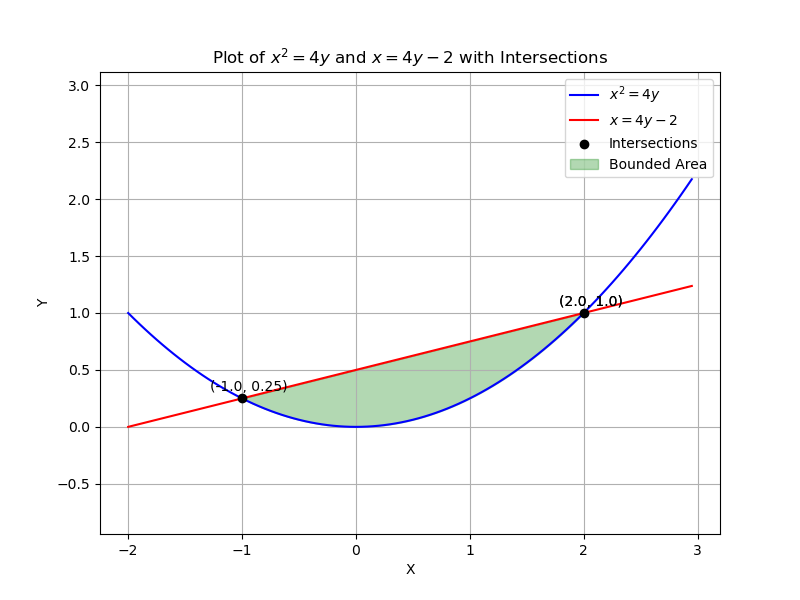
\includegraphics[width=0.7\textwidth]{Fig/fig.png}
	\caption{Line and Vectors}
	\label{fig:4-4.2-13 - Figure -1}
\end{center}
\end{figure}
\end{document}


